\documentclass[10pt]{amsart}
\usepackage[margin=1.4in]{geometry}
\usepackage{amssymb,amsmath,enumitem,url}
\usepackage{graphicx,subfig}
\graphicspath{ {./images/} }

\newcommand{\D}{\mathrm{d}}
\newcommand{\I}{\mathrm{i}}
\DeclareMathOperator{\E}{e}
\DeclareMathOperator{\OO}{O}
\DeclareMathOperator{\oo}{o}
\DeclareMathOperator{\erfc}{erfc}
\DeclareMathOperator{\real}{Re}
\DeclareMathOperator{\imag}{Im}
\usepackage{tikz}
\usepackage[framemethod=tikz]{mdframed}
\theoremstyle{nonumberplain}

\mdtheorem[innertopmargin=-5pt]{sol}{Solution}
%\newmdtheoremenv[innertopmargin=-5pt]{sol}{Solution}

\begin{document}
\pagestyle{empty}

\newcommand{\mline}{\vspace{.2in}\hrule\vspace{.2in}}

\noindent
\text{Hunter Lybbert} \\
\text{Student ID: 2426454} \\
\text{01-16-25} \\
\text{AMATH 502:} \\
\text{Dynamical Systems and Chaos} \\
% header containing your name, student number, due date, course, and the homework number as a title.

\title{\bf {Homework 1} }


\maketitle
\noindent
Exercises come from \textit{Nonlinear Dynamics and Chaos by Steven H. Strogatz}
\mline
\begin{enumerate}[label={\bf {\arabic*}:}]
\item 2.2.3 \\
\textit{Solution:}
Looking closely at the DS $\dot x = x - x^3$, we can recognize there are three fixed points at $x^* = -1, 0, 1$.
Now we can look at the plots in Figure \ref{fig:f1}, to identify that $x^* = -1, 1$ are stable fixed points and $x^* = 0$ is unstable.
\begin{figure}[h]
	\centering
	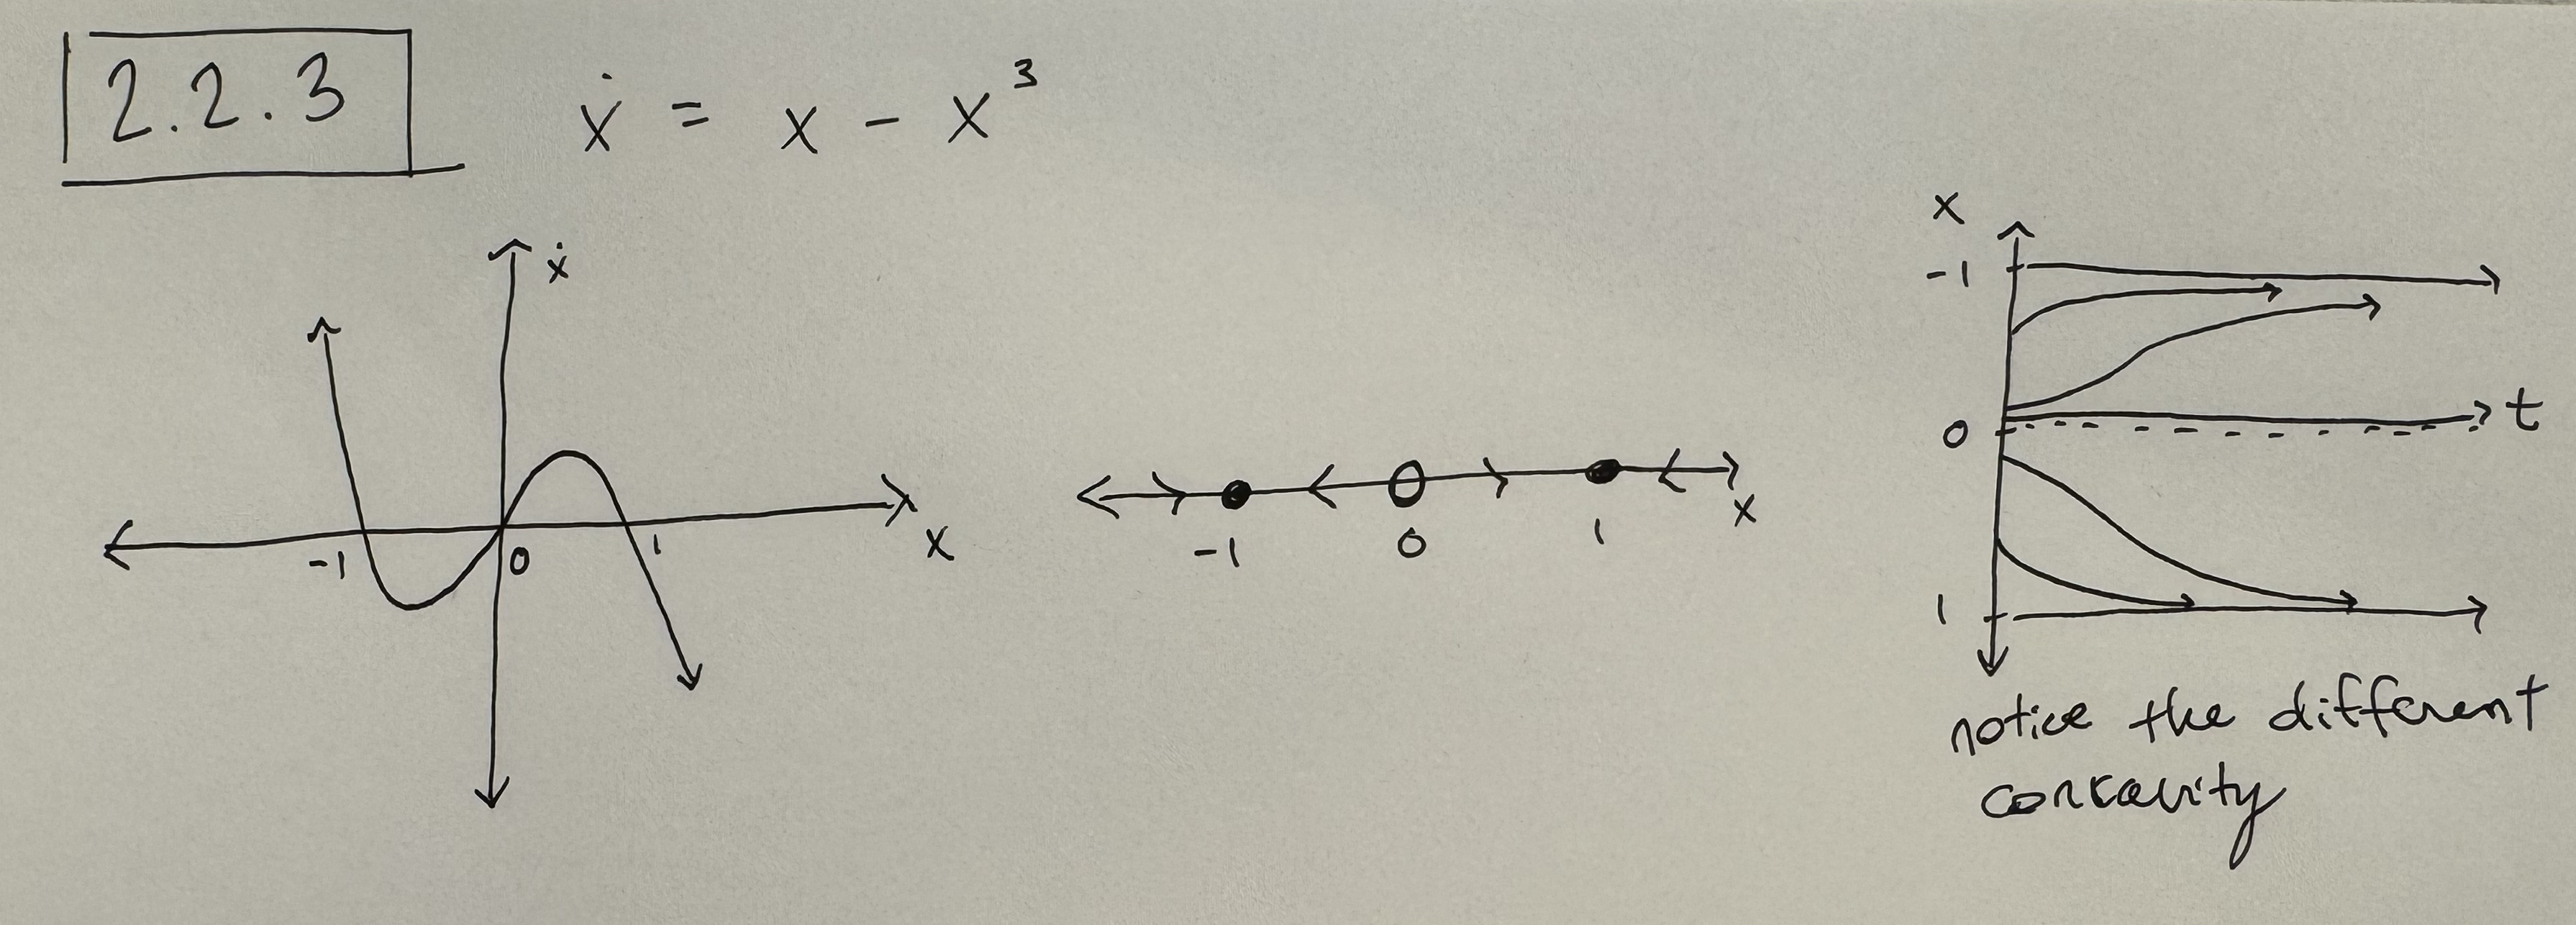
\includegraphics[width=1\textwidth]{2_2_3.png}
 	\caption{We have sketched the vector field on the real line, identified all three fixed points, classified their stability and sketched the $x(t)$ for different initial conditions.}\label{fig:f1}
\end{figure}

\qed \\

\newpage

\item 2.2.7 \\
\textit{Solution:} Looking at the DS $\dot x = \E^x - \cos x$ is tricky so let's plot in Figure \ref{fig:f2} each of $\E^x$ and $\cos x$ on the same plot to determine where the fixed points are and what their stability is.
Notice, the two functions intersect at $x = 0$ and infinitely more points as $x \rightarrow - \infty$.
Since $\E^x$ is decaying to 0 as $x \rightarrow - \infty$ the points at which the two functions intersect approach odd multiples of $\pi/2$ such that the fixed points can be written as $x^* = 0$ and $x^* \approx - \frac {2k + 1}{2}$ for the integer $k$ which is sufficiently less than 0, denoted as $k << 0$. \\

\noindent
Furthermore, note that to the right of the fixed point $x^* = 0$ we have that $\E^x > \cos x$, therefore $\E^x - \cos x < 0$ and the flow is to the right in this interval. 
Finally, note as depicted in the graph in Figure \ref{fig:f2}, that the oscillating nature of the $\cos$ function we end up with alternating flow directions and thus with alternating stability for the fixed points.
So $x^* = 0$ is an unstable fixed point, and each fixed point alternates stability as $x \rightarrow - \infty$ .
\begin{figure}[h]
	\centering
	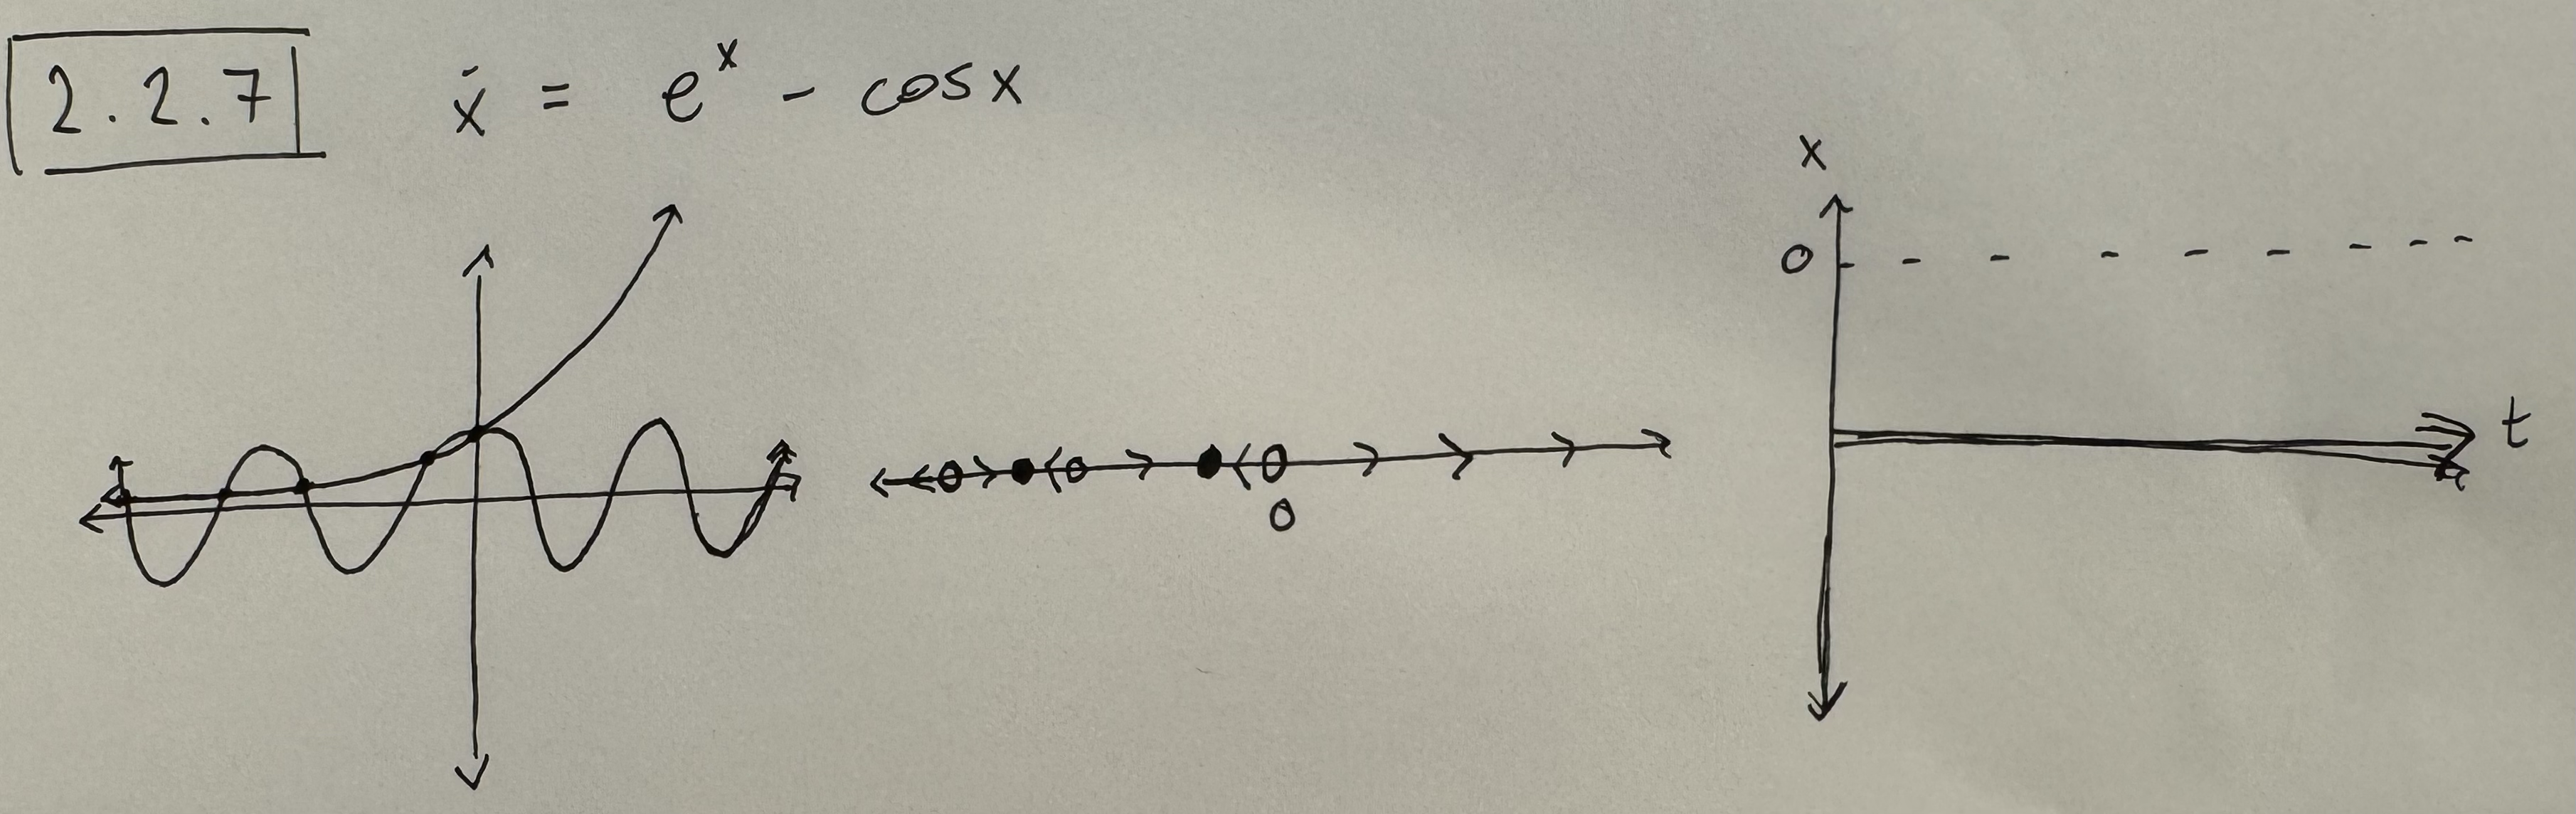
\includegraphics[width=1\textwidth]{2_2_7.png}
 	\caption{We have sketched the vector field on the real line, identified the approximate location of all the fixed points, and classified their stability (which is alternating stable and unstable). I am not actually going to come back and fill in the sketch of $x(t)$ for different initial conditions since there are an unending number of fixed points and each has two concavities due to the alternating stability and oscillating nature of the $\cos$ function.}\label{fig:f2}
\end{figure}

\qed \\

\newpage

\item 2.2.8 \\
\textit{Solution:} \\
Based on the given flow diagram $\dot x = x(x + 1)^2(x - 2)$.
Now to verify that this satisfies the criteria we are given I will plug in values in the ranges given and verify they match the expected flow direction.
We also have depicted this in Figure \ref{fig:f3}

\begin{align*}
\dot x &= \left. x(x + 1)^2(x - 2) \right|_{x = -2} \\
\dot x &= -2(-2 + 1)^2(-2 - 2) \\
\dot x &= -2(-1)^2(-4) \\
\dot x &= 8 > 0 \\ \\
\dot x &= \left. x(x + 1)^2(x - 2) \right|_{x = -.5} \\
\dot x &= -.5(-.5 + 1)^2(-.5 - 2) \\
\dot x &= -.5(.5)^2( -2.5) > 0 \\ \\
\dot x &= \left. x(x + 1)^2(x - 2) \right|_{x = 1} \\
\dot x &= 1(1 + 1)^2(1 - 2) \\
\dot x &= 1(1 + 1)^2(-1) < 0 \\ \\
\dot x &= \left. x(x + 1)^2(x - 2) \right|_{x = 3} \\
\dot x &= 3(3 + 1)^2(3 - 2) \\
\dot x &= 3(3 + 1)^2(1) > 0
\end{align*}

\begin{figure}[h]
	\centering
	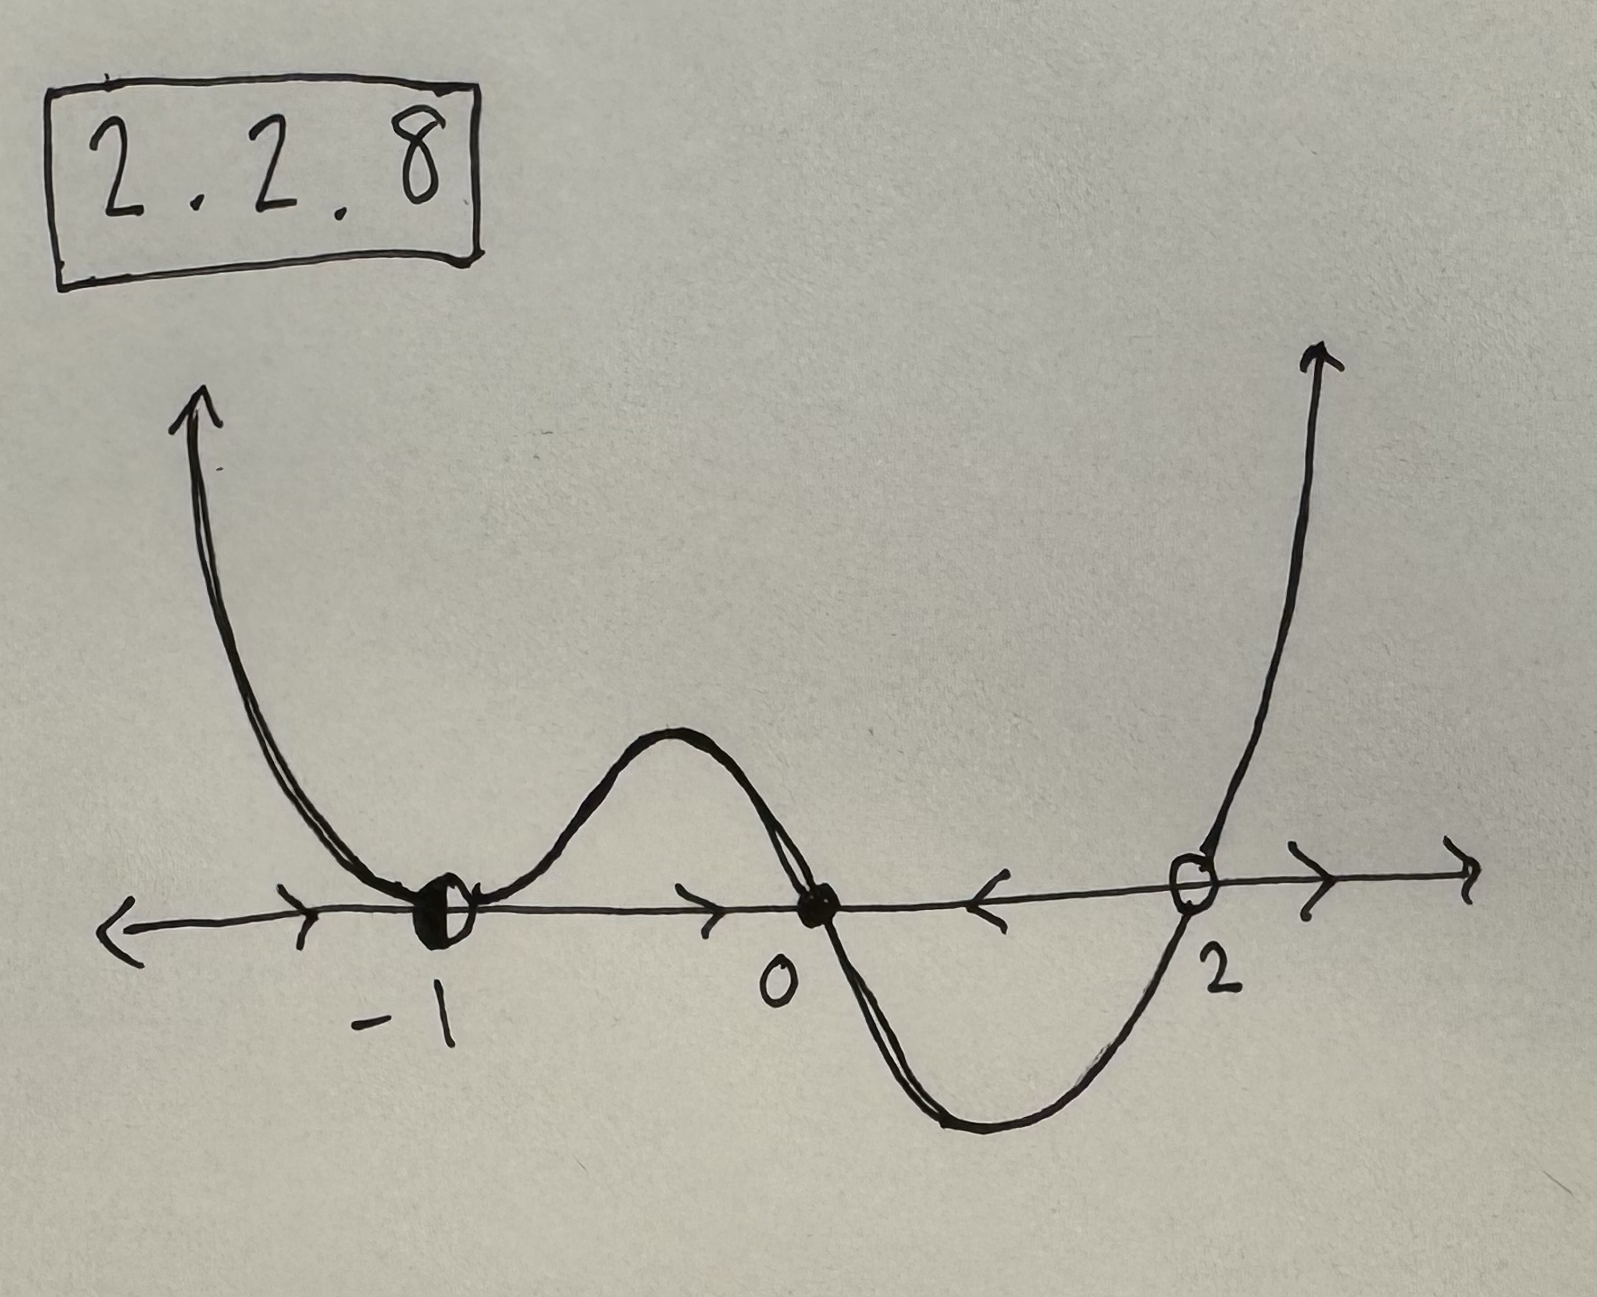
\includegraphics[height=2in]{2_2_8.png}
 	\caption{On the $x$-axis I have written the provided phase diagram and plotted over it one possible polynomial which satisfies the required flows.}\label{fig:f3}
\end{figure}

\qed \\

\newpage

\item 2.2.10 \\
Find an equation $\dot x = f(x)$ with the stated properties, or if there are no examples, explain why not. \\

\noindent
\begin{enumerate}
\item Every real number is a fixed point. \\
\textit{Solution:} Let $\dot x = f(x) = 0$ be a constant function. \\

\item Every integer is a fixed point and there are no others. \\
\textit{Solution:} Let $\dot x = f(x) = \sin(\pi x)$. \\

\item Precisely three fixed points, and all three are stable. \\
\textit{Solution:} This is not possible since a fixed point has to have a negative slope at that point and you can't cross the $x$-axis from the upper left to the lower right 3 times without having crossed the $x$-axis once in between to return above the $x$-axis.
This would force there to be an additional fixed point or for one of the 3 fixed points to be unstable (namely the one in between). \\

\item There are no fixed points. \\
\textit{Solution:} Let $\dot x = f(x) = \E^x$. \\

\item There are precisely 100 fixed points. \\
\textit{Solution:} Let $x_i \in \mathbb R$ for $i = 1, 2, ..., 100$ and $x_i \neq x_j$ for $i \neq j$.
Therefore we can say 
$$\dot x = f(x) = \prod_{i=1}^{100} (x - x_i).$$
\end{enumerate}

\qed \\
\newpage

\item 2.2.13 (a,b,c,d) \\
\begin{enumerate}
\item $m \dot v = mg - kv^2$ with initial condition $v(0) = 0$ \\

\noindent
\textit{Solution:} \\
Let's begin by dividing by $m$ and factoring out a $g$ term.
\begin{align*}
m \dot v &= mg - kv^2 \\
\dot v &= g - \frac{kv^2}{m} \\
\dot v &= g\left( 1 - \frac{kv^2}{gm}\right).
\end{align*}
Now rewriting $\dot v$ as the derivative of $v$ with respect to $t$ we have
\begin{align*}
\frac{\D v}{\D t} &= g\left( 1 - \frac{kv^2}{gm}\right) \\
\frac{1}{\left( 1 - \frac{kv^2}{gm}\right)}\D v &= g \D t \\
\int \frac{1}{\left( 1 - \sqrt{\frac{k}{gm}}v\right)\left( 1 + \sqrt{\frac{k}{gm}}v\right)}\D v &= \int g \D t.
\end{align*}
Now, we can do partial fractions on the left and integrate both sides
\begin{align*}
\int \frac{1}{\left( 1 - \sqrt{\frac{k}{gm}}v\right)\left( 1 + \sqrt{\frac{k}{gm}}v\right)}\D v &= \int g \D t \\
\int \frac{1/2}{\left( 1 - \sqrt{\frac{k}{gm}}v\right)}\D v
	+ \int \frac{1/2}{\left( 1 + \sqrt{\frac{k}{gm}}v\right)}\D v
	 &= g t + C \\
- \frac 1 2 \sqrt{\frac {gm}{k}}\log\left( 1 - \sqrt{\frac{k}{gm}}v\right)
	+ \frac 1 2 \sqrt{\frac {gm}{k}}\log\left( 1 + \sqrt{\frac{k}{gm}}v\right)
	 &= g t + C \\
\frac 1 2 \sqrt{\frac {gm}{k}}\Bigg( \log \left( 1 + \sqrt{k/(gm)} \: v\right) 
	- \log \left( 1 - \sqrt{k/(gm)} \: v\right) \Bigg)
	 &= g t + C
\end{align*}
Interesting ... now I need to input the initial condition \\
\begin{align*}
\frac 1 2 \sqrt{\frac {gm}{k}}\Bigg( \log \left( 1 + \sqrt{k/(gm)} \: 0\right) 
	- \log \left( 1 - \sqrt{k/(gm)} \: 0\right) \Bigg)
	 &= g 0 + C \\
\frac 1 2 \sqrt{\frac {gm}{k}}\Bigg( \log \left( 1 \right) 
	- \log \left( 1 \right) \Bigg) &= C \\
	0 &= C.
\end{align*}
Plugging this in and simplifying we have
\begin{align*}
\frac 1 2 \sqrt{\frac {gm}{k}}\Bigg( \log \left( 1 + \sqrt{k/(gm)} \: v\right) 
	- \log \left( 1 - \sqrt{k/(gm)} \: v\right) \Bigg)
	 &= g t \\
\log \left( \frac {1 + \sqrt{k/(gm)} \: v}{1 - \sqrt{k/(gm)} \: v}\right) 
	 &= 2 g t \sqrt{k/(gm)}.
\end{align*}
Now we can exponentiate and solve for $v$
\begin{align*}
\frac {1 + \sqrt{k/(gm)} \: v}{1 - \sqrt{k/(gm)} \: v}
	 &= \E^{2 g t \sqrt{k/(gm)}} \\
1 + \sqrt{k/(gm)} \: v
	 &= \E^{2 g t \sqrt{k/(gm)}}(1 - \sqrt{k/(gm)} \: v) \\
1 + \sqrt{k/(gm)} \: v 
	 &= \E^{2 g t \sqrt{k/(gm)}} - \sqrt{k/(gm)} \: v \E^{2 g t \sqrt{k/(gm)}} \\
\sqrt{k/(gm)} \: v +  \sqrt{k/(gm)} \: v \E^{2 g t \sqrt{k/(gm)}}
	 &= \E^{2 g t \sqrt{k/(gm)}} - 1 \\
v &= \frac {\E^{2 g t \sqrt{k/(gm)}} - 1}{\sqrt{k/(gm)} +  \sqrt{k/(gm)} \E^{2 g t \sqrt{k/(gm)}}}.
\end{align*}
Some final simplifications gives us
\begin{align*}
v &= \frac 1 {\sqrt{k/(gm)}}\frac {\E^{2 g t \sqrt{k/(gm)}} - 1}{1 +  \E^{2 g t \sqrt{k/(gm)}}} \\
v &= \sqrt{\frac {gm}{k}} \left( \frac {\E^{2 g t \sqrt{k/(gm)}} - 1}{\E^{2 g t \sqrt{k/(gm)}}+ 1} \right).
\end{align*}
Therefore our final analytical solution is 
$$
v = \sqrt{\frac {gm}{k}} \left( \frac {\E^{2 g t \sqrt{k/(gm)}} - 1}{\E^{2 g t \sqrt{k/(gm)}}+ 1} \right).
$$
\qed \\

\item Determine the limit of $v(t)$ as $t\rightarrow \infty$.
We will need to utilize L'Hôpital's rule since the numerator and the denominator go to infinity.
\begin{align*}
\lim_{t\rightarrow \infty} \sqrt{\frac {gm}{k}} \left( \frac {\E^{2 g t \sqrt{k/(gm)}} - 1}{\E^{2 g t \sqrt{k/(gm)}}+ 1} \right)
	&= \lim_{t\rightarrow \infty} \sqrt{\frac {gm}{k}} \left( \frac {2 g t \sqrt{k/(gm)}\E^{2 g t \sqrt{k/(gm)}}}{2 g t \sqrt{k/(gm)}\E^{2 g t \sqrt{k/(gm)}}} \right) \\
	&= \lim_{t\rightarrow \infty} \sqrt{\frac {gm}{k}} \\
	&= \sqrt{\frac {gm}{k}}.
\end{align*}
Therefore, the terminal velocity is $\sqrt{\frac {gm}{k}}$. \\
\qed \\

\newpage

\item Graphical argument. \\

\textit{Solution:}
Beginning with $m \dot v = mg - kv^2$ we have

$$\dot v = g - \frac k  m v^2.$$

By inspection we can see that $\dot v = g - \frac k  m v^2 = (\sqrt{\frac {gm}{k}} - v)(\sqrt{\frac {gm}{k}} + v) = 0$.
Therefore, the fixed points are $v = \pm \sqrt{\frac {gm}{k}}$.

\begin{figure}[h]
	\centering
	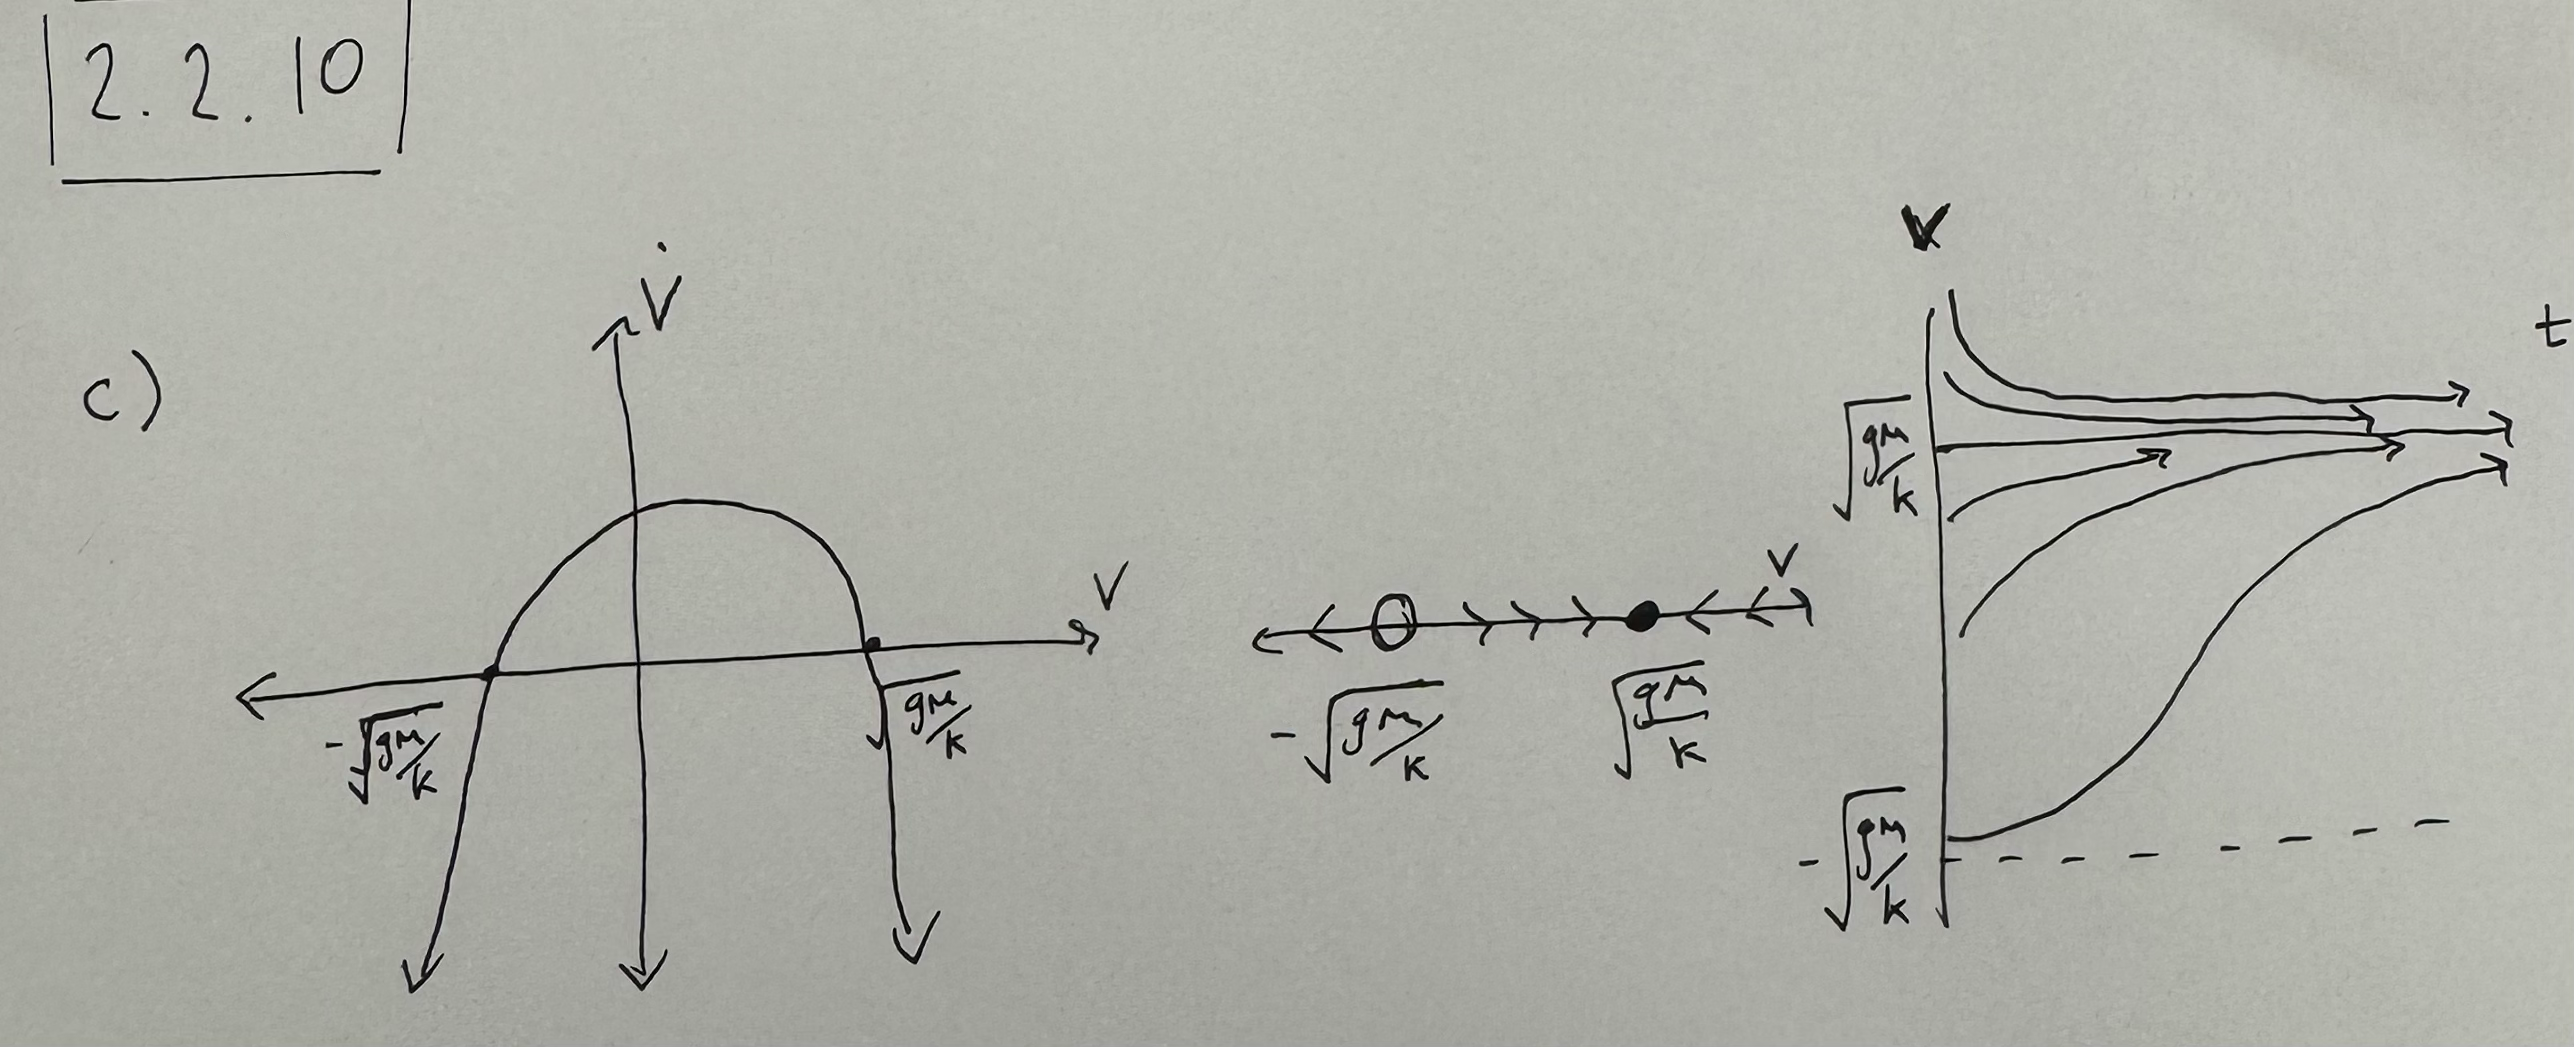
\includegraphics[height=2in]{2_2_13_c.png}
 	\caption{We have sketched the vector field on the real line, identified the location of all the fixed points, classified their stability, and sketched the $x(t)$ for different initial conditions (ignore the typo in the photograph this is for 2.2.13 c) not 2.2.10 c) as it is written)}\label{fig:f4}
\end{figure}

\qed \\

\item Calculate the average velocity. \\

\noindent
\textit{Solution:}
$$\frac{31,400 - 2,100 {\rm ft}}{116 {\rm s}} = \frac{29,300 {\rm ft} }{116 {\rm s}} \approx 253 {\rm ft}/{\rm s} = 172 {\rm mph}.$$
\qed \\

\end{enumerate}

\newpage

\item 2.3.2 Analyze the DS governed by $\dot x = k_1 a x - k_{-1} x^2$ \\

\begin{enumerate}
\item Find all the fixed points and classify their stability \\
\textit{Solution:} \\

\noindent
Notice $\dot x$ has fixed points at $x^* = 0, \frac {k_1 a}{k_{-1}}$, since
\begin{align*}
\dot x &= k_1 a x - k_{-1} x^2 \\
\dot x &= x (k_1 a - k_{-1} x).
\end{align*}
Then $\dot x = x (k_1 a - k_{-1} x) = 0$ implies the above fixed points.
We will analyze this graphically.
Looking at Figure \ref{fig:f5} makes it obvious that $x^* = 0$ is unstable and $x^* = \frac {k_1 a}{k_{-1}}$ is stable.

\begin{figure}[h]
	\centering
	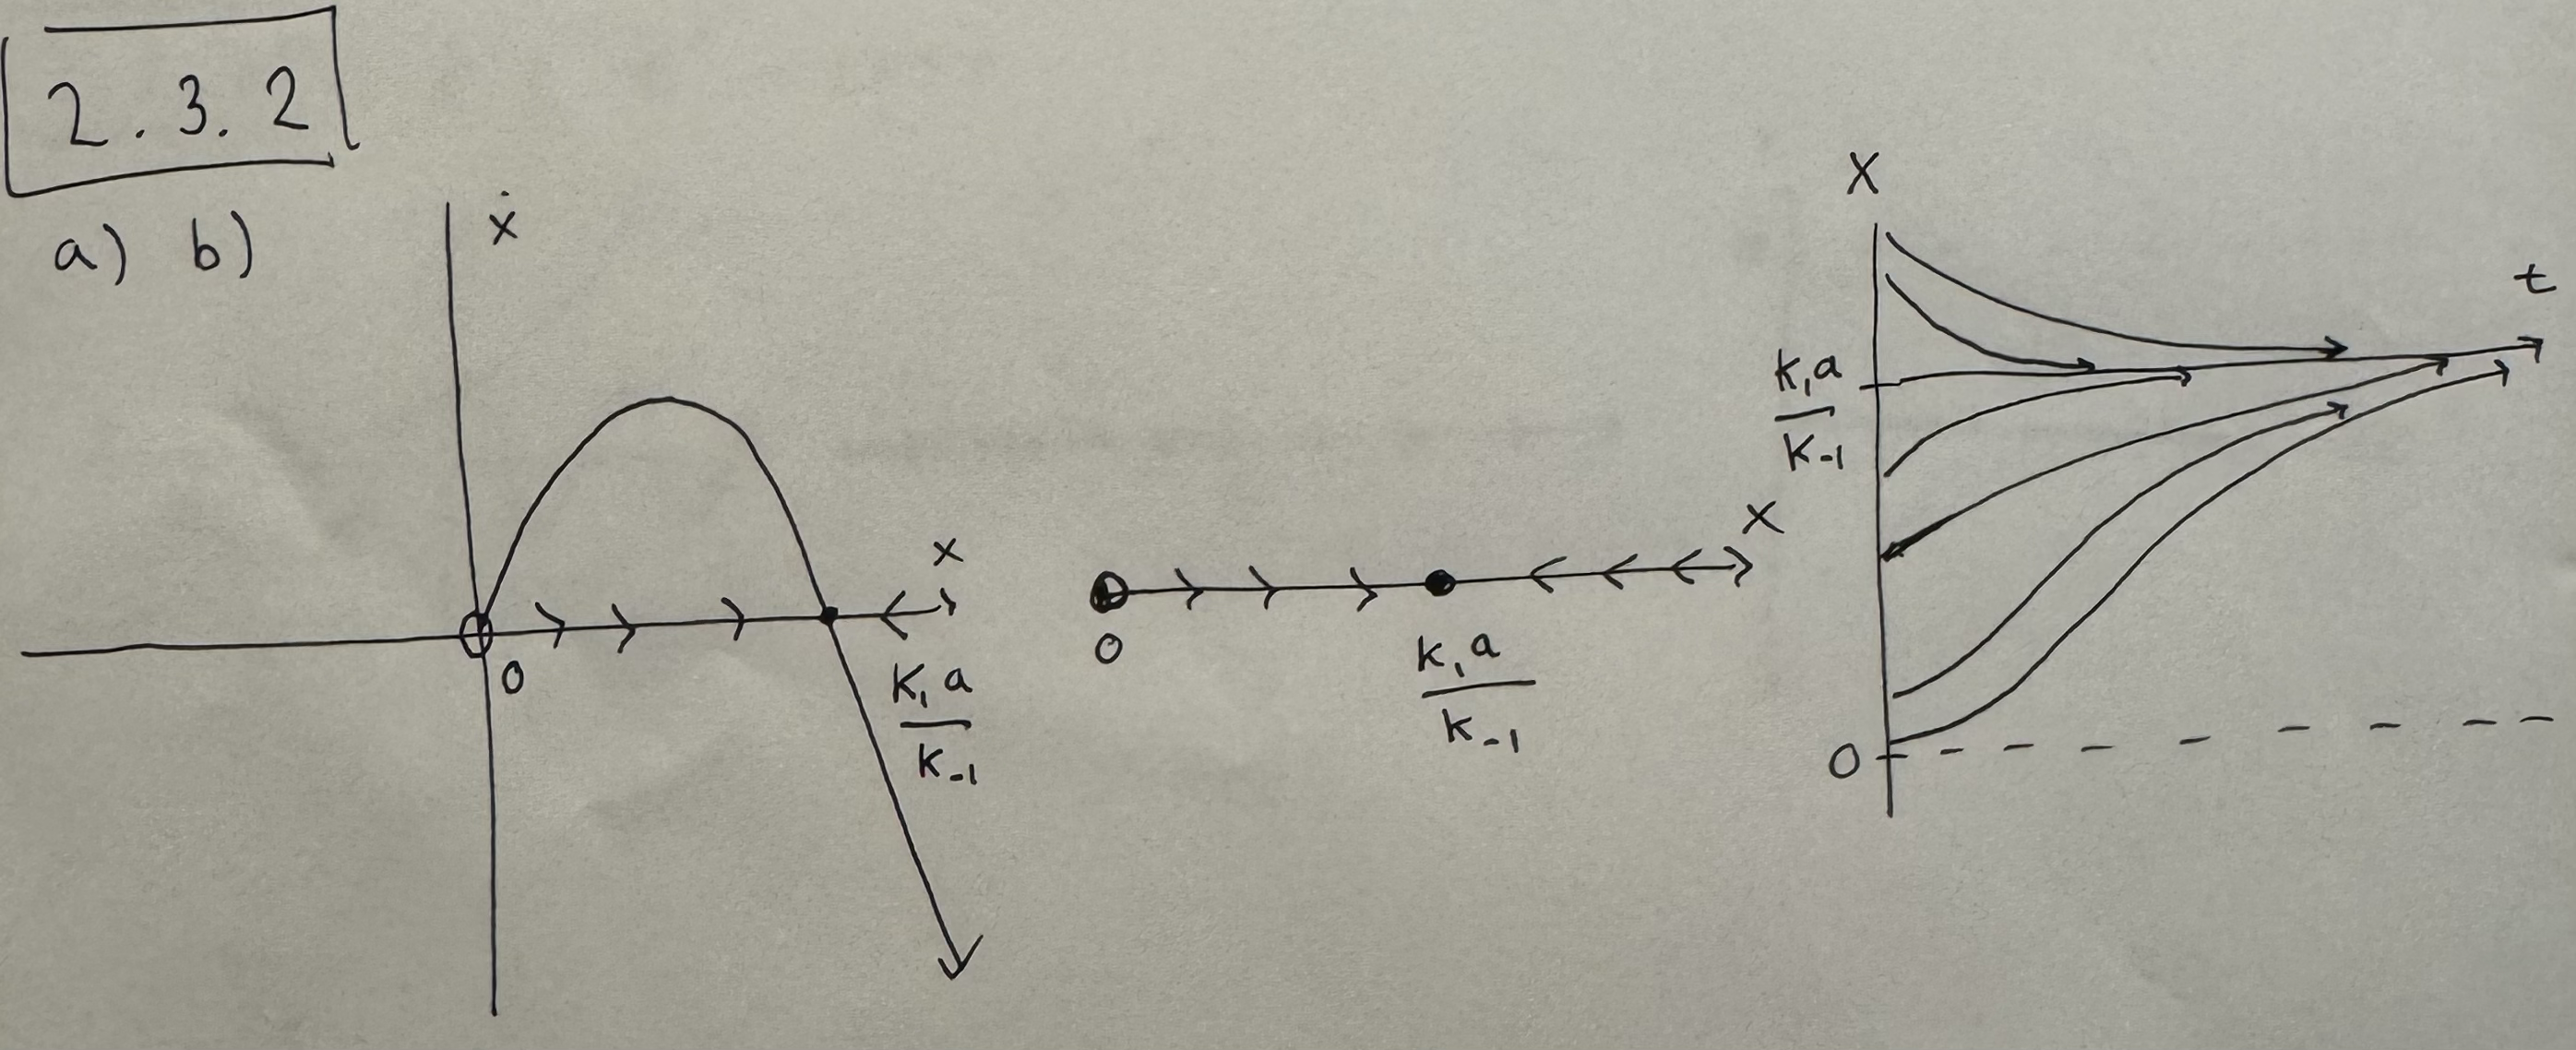
\includegraphics[height=2in]{2_3_2.png}
 	\caption{We have sketched the vector field on the real line, identified the location of all the fixed points, classified their stability, and sketched the $x(t)$ for different initial conditions.}\label{fig:f5}
\end{figure}

\qed \\

\item Sketch the graph of $x(t)$ for various initial values of $x_0$. \\

\noindent
\textit{Solution:} See Figure \ref{fig:f5} \\
\qed \\

\end{enumerate}

\newpage

\item 2.3.6  We are looking at the model governed by $\dot x  = s(1 - x) x^a - (1 - s)x(1 - x)^a$ \\

\begin{enumerate}

\item Show that this equation for $\dot x$ has three fixed points. \\

\noindent
\textit{Solution:} \\
We fist begin by factoring the expression on the rhs first to get
$$
\dot x  = x(1 - x)\big(sx^{a-1} - (1 - s)(1 - x)^{a - 1}\big).
$$
Now we know the fixed points occur at $x^* = 0, 1$ and when the third factor is equal to 0.
Let's algebraically solve for this third fixed point, by setting it equal to zero and solving for $x$.
\begin{align*}
sx^{a-1} - (1 - s)(1 - x)^{a - 1} &= 0 \\
sx^{a-1} - (1 - x)^{a - 1} + s(1 - x)^{a - 1} &= 0 \\
s \big( x^{a-1} + (1 - x)^{a - 1}\big) &= (1 - x)^{a - 1} \\
s \frac {\big( x^{a-1} + (1 - x)^{a - 1}\big)}{x^{a - 1}} &= \frac {(1 - x)^{a - 1}}{x^{a - 1}} \\
s \left( 1 +  \left(\frac {1 - x}{x} \right)^{a - 1} \right) &= \left(\frac {1 - x}{x} \right)^{a - 1} \\
s &= \left(\frac {1 - x}{x} \right)^{a - 1} - s \left(\frac {1 - x}{x} \right)^{a - 1} \\
s &= (1 - s)\left(\frac {1 - x}{x} \right)^{a - 1} \\
\left( \frac s {1 - s} \right)^{\frac 1 {a - 1}} &= \frac {1 - x}{x} \\
x + x \left( \frac s {1 - s} \right)^{\frac 1 {a - 1}} &= 1 \\
x\left( 1 + \left( \frac s {1 - s} \right)^{\frac 1 {a - 1}}\right) &= 1 \\
x &= \frac 1 { 1 + \left( \frac s {1 - s} \right)^{\frac 1 {a - 1}}}.
\end{align*}
Therefore we have there are 3 distinct fixed points. \\
\qed \\

\newpage
 

\item Show that for all $a > 1$, the fixed points at $x = 0$ and $x = 1$ are both stable. \\

\noindent
\textit{Solution:} \\
Let's do so by LSA.
So we first need to take the derivative of $f$ with respect to $x$ from
$$
\dot x = f(x)  = s(1 - x) x^a - (1 - s)x(1 - x)^a.
$$
Then,
\begin{align*}
f^\prime(x) &= \frac {d f}{d x} \big( s(1 - x) x^a - (1 - s)x(1 - x)^a \big) \\
	&= \frac {d f}{d x} s(1 - x) x^a - \frac {d f}{d x} (1 - s)x(1 - x)^a \\
	&= - s x^a + sa (1 - x) x^{a - 1} - (1 - s)(1 - x)^a + (1 - s)x(1 - x)^{a - 1}.
\end{align*}
Now we can evaluate this at $x^* = 0$ and $x^* = 1$ as follows,
\begin{align*}
f^\prime(x^* = 0) &= \left. - s x^a + sa (1 - x) x^{a - 1} - (1 - s)(1 - x)^a + (1 - s)x(1 - x)^{a - 1} \right|_0 \\
	&= - s 0^a + sa (1 - 0) 0^{a - 1} - (1 - s)(1 - 0)^a + (1 - s)0(1 - 0)^{a - 1} \\
	&= - (1 - s)1^a \\
	&= s - 1 \leq 0.
\end{align*}

Therefore, $f^\prime(x^* = 0) \leq 0$ since $s$ could be equal to 1.
Assuming $s < 1$ we have that the fixed point $x^* = 0$ is stable by LSA.

\begin{align*}
f^\prime(x^* = 1) &= \left. - s x^a + sa (1 - x) x^{a - 1} - (1 - s)(1 - x)^a + (1 - s)x(1 - x)^{a - 1} \right|_0 \\
	&= - s 1^a + sa (1 - 1) 1^{a - 1} - (1 - s)(1 - 1)^a + (1 - s)1(1 - 1)^{a - 1} \\
	&= - s \leq 0.
\end{align*}
Therefore, $f^\prime(x^* = 1) \leq 0$ since $s$ could be equal to 0.
Assuming $s > 0$ we have that the fixed point $x^* = 1$ is stable by LSA. \\
\qed \\

\item Show that the third fixed point, $0 < x^* < 1$, is unstable. \\

\noindent
\textit{Solution:} We know there are three fixed points by part a), by 2.2.10 we established that a DS with precisely three fixed points can't all be stable, finally by part b) we know that $x^* = 0 \; {\rm and} \; 1$ are stable then the fixed point which lies within the interval $0 < x^* < 1$ must be unstable. \\
\qed \\

\end{enumerate}

\newpage

\item 2.4.7 Use LSA to classify the fixed points of the system, $\dot x = ax - x^3$. If linear stability analysis fails because $f^\prime (x^*) = 0$, use a graphical argument to decide the stability. \\


\begin{enumerate}

\item Where $a > 0$ \\

\noindent
\textit{Solution:} The fixed points are going to be given by $x^* = 0, \pm \sqrt{a}$ which are all real valued fixed points since $a > 0$.
Now to use LSA we need to calculate the derivative of $f$ with respect to $x$, therefore we have
$$
f^\prime (x) = a - 3x^2.
$$
Then 
$$f^\prime (x^* = 0) = a > 0$$
thus $x^* = 0$ is unstable.
Lastly
$$f^\prime (x^* = \pm \sqrt a) = a - 3a = -2a < 0$$
thus both $\pm \sqrt a $ are stable.

\qed \\

\item Where $a = 0$ \\

\noindent
\textit{Solution:} In this case the system reduces to $\dot x = -x^3$ which only has one fixed point at $x^* = 0$. 
The derivative becomes $f^\prime(x) = -3x^2$ which evidently gives us $f^\prime(x^*= 0) = 0$ therefore LSA is inconclusive and we will analyze graphically.
By the analysis in Figure \ref{fig:f6} we can see that $x^* = 0$ is a stable fixed point.

\begin{figure}[h]
	\centering
	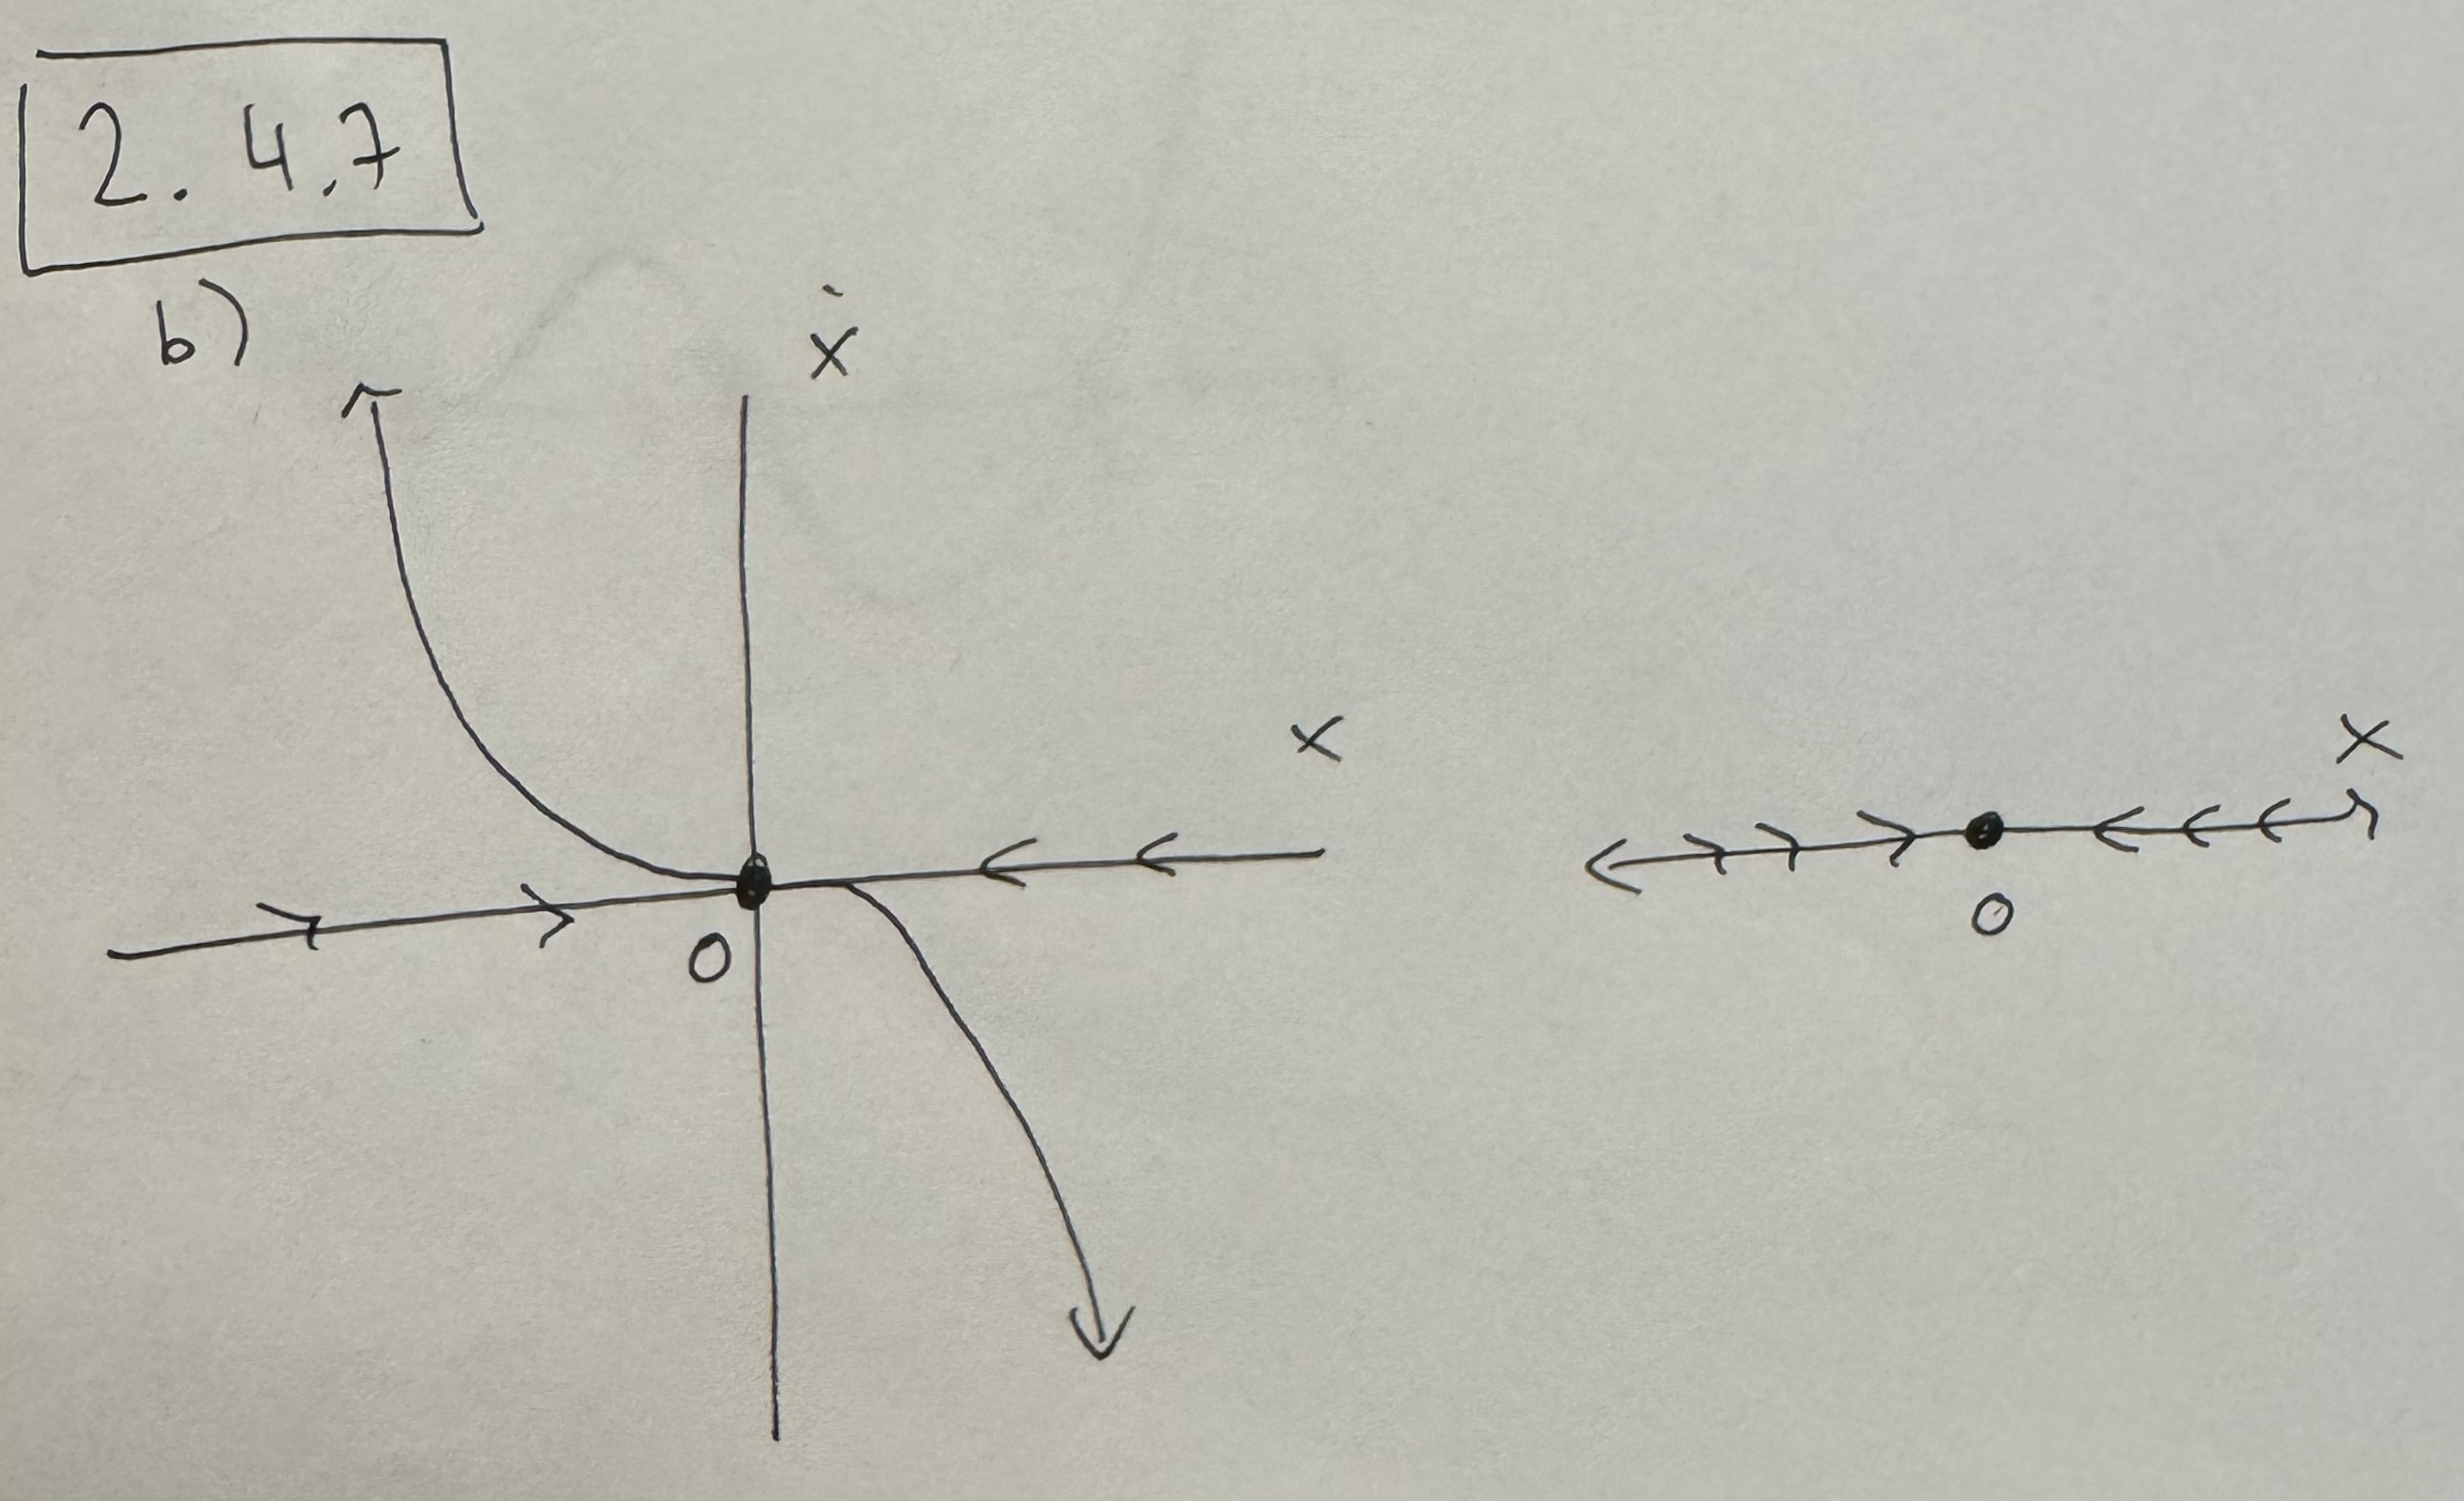
\includegraphics[height=1.5in]{2_4_7.png}
 	\caption{We have sketched the vector field on the real line, identified the location of all the fixed points, and classified their stability.}\label{fig:f6}
\end{figure}

\item Where $a < 0$ \\

\noindent
\textit{Solution:} Again the fixed points are at $x^* = 0, \pm \sqrt a$. However, since $a < 0$ and we are not currently handling non-real fixed points, we conclude there is just one fixed point at $x^* = 0$. \\

\noindent
Furthermore, performing LSA using the $f^\prime(x) = a - 3x^2$, gives us
$$f^\prime (x^* = 0) = a < 0, $$
thus $x^* = 0$ is a stable fixed point in this scenario.

\qed \\

\end{enumerate}

\end{enumerate}

\end{document}

%%% Local Variables:
%%% mode: latex
%%% TeX-master: t
%%% End:
